\documentclass[tikz]{standalone}
\usepackage{cancel}
\usepackage{fontspec}
\setmonofont[Scale=MatchLowercase]{DejaVu Sans Mono}
\usetikzlibrary{arrows.meta}

\begin{document}
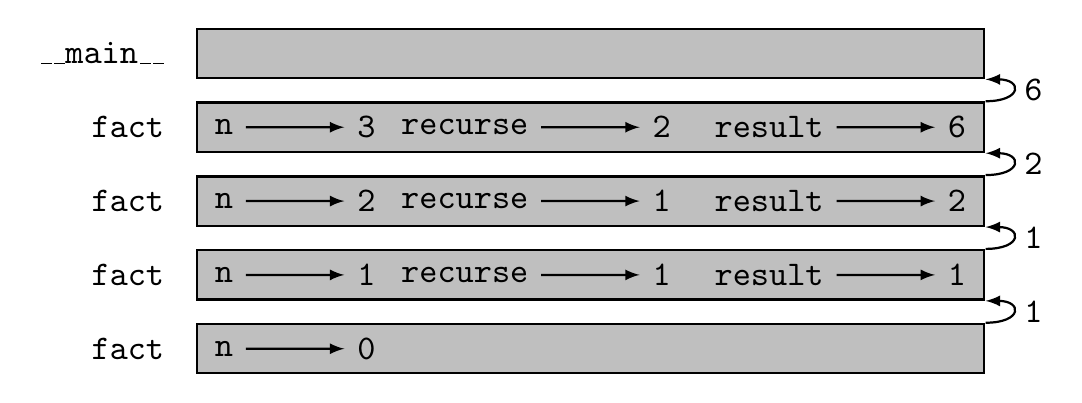
\begin{tikzpicture}[thick, scale=1.25, transform shape]
$\node[anchor=east] at(-4.2,0){\tt \_\_main\_\_};
\node[draw, fill=lightgray, minimum width=8cm, minimum height=0.5cm](c0){};
\node[anchor=east] at(-4.2,-0.75){\tt fact};
\node[draw, fill=lightgray, minimum width=8cm, minimum height=0.5cm](c1) at(0,-0.75){};
\node[anchor=east] (n1) at(-3.5, -0.75) {\tt n};
\node[anchor=west] (n1v) at (-2.5, -0.75) {\tt 3};
\node[anchor=east] (r1) at(-0.5, -0.75) {\tt recurse};
\node[anchor=west] (r1v) at (0.5, -0.75) {\tt 2};
\node[anchor=east] (e1) at(2.5, -0.75) {\tt result};
\node[anchor=west] (e1v) at (3.5, -0.75) {\tt 6};
\draw[-latex] (n1) -- (n1v);
\draw[-latex] (r1) -- (r1v);
\draw[-latex] (e1) -- (e1v);
\node[anchor=east] at(-4.2,-1.5){\tt fact};
\node[draw, fill=lightgray, minimum width=8cm, minimum height=0.5cm](c2) at(0,-1.5){};
\node[anchor=east] (n1) at(-3.5, -1.5) {\tt n};
\node[anchor=west] (n1v) at (-2.5, -1.5) {\tt 2};
\node[anchor=east] (r1) at(-0.5, -1.5) {\tt recurse};
\node[anchor=west] (r1v) at (0.5, -1.5) {\tt 1};
\node[anchor=east] (e1) at(2.5, -1.5) {\tt result};
\node[anchor=west] (e1v) at (3.5, -1.5) {\tt 2};
\draw[-latex] (n1) -- (n1v);
\draw[-latex] (r1) -- (r1v);
\draw[-latex] (e1) -- (e1v);
\node[anchor=east] at(-4.2,-2.25){\tt fact};
\node[draw, fill=lightgray, minimum width=8cm, minimum height=0.5cm](c3) at(0,-2.25){};
\node[anchor=east] (n1) at(-3.5, -2.25) {\tt n};
\node[anchor=west] (n1v) at (-2.5, -2.25) {\tt 1};
\node[anchor=east] (r1) at(-0.5, -2.25) {\tt recurse};
\node[anchor=west] (r1v) at (0.5, -2.25) {\tt 1};
\node[anchor=east] (e1) at(2.5, -2.25) {\tt result};
\node[anchor=west] (e1v) at (3.5, -2.25) {\tt 1};
\draw[-latex] (n1) -- (n1v);
\draw[-latex] (r1) -- (r1v);
\draw[-latex] (e1) -- (e1v);
\node[anchor=east] at(-4.2,-3){\tt fact};
\node[draw, fill=lightgray, minimum width=8cm, minimum height=0.5cm](c4) at(0,-3){};
\node[anchor=east] (n1) at(-3.5, -3) {\tt n};
\node[anchor=west] (n1v) at (-2.5, -3) {\tt 0};
\draw[-latex] (n1) -- (n1v);
\draw [-latex](c4.north east) to[out=0,in=0,distance=0.375cm] (c3.south east);
\draw [-latex](c3.north east) to[out=0,in=0,distance=0.375cm] (c2.south east);
\draw [-latex](c2.north east) to[out=0,in=0,distance=0.375cm] (c1.south east);
\draw [-latex](c1.north east) to[out=0,in=0,distance=0.375cm] (c0.south east);
\node [right of=c4, xshift=3.5cm, yshift=0.375cm] {\tt 1};
\node [right of=c3, xshift=3.5cm, yshift=0.375cm] {\tt 1};
\node [right of=c2, xshift=3.5cm, yshift=0.375cm] {\tt 2};
\node [right of=c1, xshift=3.5cm, yshift=0.375cm] {\tt 6};
$
\end{tikzpicture}
\end{document}
